\documentclass[10pt]{article}
\usepackage[utf8]{inputenc}
\usepackage[T1]{fontenc}
\usepackage{amsmath}
\usepackage{amsfonts}
\usepackage{amssymb}
\usepackage{mhchem}
\usepackage{stmaryrd}
\usepackage{graphicx}
\usepackage[export]{adjustbox}
\graphicspath{ {./images/} }

\title{GNP }


\author{Partie I - Introduction}
\date{}


\begin{document}
\maketitle


\section*{INFORMATIQUE }
Mercredi 6 mai : 8 h - 11 h

N.B. : le candidat attachera la plus grande importance à la clarté, à la précision et à la concision de la rédaction. Si un candidat est amené a repérer ce qui peut lui sembler être une erreur d'énoncé, il le signalera sur sa copie et devra poursuivre sa composition en expliquant les raisons des initiatives qu'il a été amené a prendre.

\section{RAPPEL DES CONSIGNES}
\begin{itemize}
  \item Utiliser uniquement un stylo noir ou bleu foncé non effaçable pour la rédaction de votre composition ; d'autres couleurs, excepté le vert, peuvent être utilisées, mais exclusivement pour les schémas et la mise en évidence des résultats.

  \item Ne pas utiliser de correcteur.

  \item Ecrire le mot FIN a la fin de votre composition.

\end{itemize}
\section{Les calculatrices sont interdites}
\section{Le sujet est composé de trois parties indépendantes.}
L'épreuve est à traiter en langage Python. La syntaxe de Python est rappelée en Annexe, page $8 \mathrm{du}$ Document Réponse.

Les différents algorithmes doivent être rendus dans leur forme définitive sur le document réponse dans l'espace réservé à cet effet en respectant les éléments de syntaxe du langage (les brouillons ne sont pas acceptés).

La réponse ne doit pas se cantonner à la rédaction de l'algorithme sans explication, les programmes doivent être expliqués et commentés.

\section{Énoncé : page 1 à page 12}
Document réponse et Annexe : page 1 à page 8

Seul le Document Réponse est à rendre.

\section*{Détection d'obstacles par un sonar de sous-marin }

Pour détecter des obstacles sous l'eau, en l'absence de visuel direct, les sous-marins sont équipés de sonars. L'onde ultrasonore émise par le sonar est réfléchie sur l'obstacle et le signal en retour est détecté et analysé pour obtenir la distance de l'obstacle au sous-marin. Une des difficultés rencontrée lors de l'analyse du signal de retour est de déterminer si l'obstacle est une roche ou un objet métallique donc un danger potentiel.

Il existe des techniques d'aide à la décision faisant partie des algorithmes dits d'Intelligence Artificielle permettant d'analyser le signal de retour d'un sonar et de déterminer de quelle nature est l'obstacle.

Objectif

L'objectif du travail proposé est de découvrir des algorithmes d'Intelligence Artificielle en s'appuyant sur ce problème de détection d'obstacle. À partir d'une base de données comportant des mesures de sonar réalisées sur des roches et sur du métal, il s'agira d'être capable de déterminer à partir d'une mesure inconnue, si l'objet situé devant le sous marin est une roche ou un objet métallique.

Le sujet abordera les points suivants :

\begin{itemize}
  \item analyse et représentation des données,

  \item construction des arbres de décisions,

  \item prédiction par la méthode « random forest ».

\end{itemize}
Dans tout le sujet, il sera supposé que les modules python numpy, matplotlib.pyplot sont déjà importés dans le programme (cf. Annexe), on utilisera donc les fonctions de ces modules sans préciser l'origine de celles-ci. Lorsqu'il est demandé de définir des vecteurs ou des matrices, il est demandé d'utiliser le type array du module numpy.

\section*{Partie II - Analyse des données }
\section{II.1 - Présentation}
Les données utilisées pour l'apprentissage de l'algorithme ont été obtenues suite à une campagne d'essais réalisés dans l'océan à partir des mesures d'un sonar situé à environ 10 mètres d'un cylindre métallique ou d'un cylindre en pierre pour différentes incidences angulaires du signal émis par le sonar.

Le signal émis par le sonar et le signal reçu sont numériques et représentés avec $N$ valeurs sur une durée totale $T_{f}$. Les variables $\mathrm{Tf}$ et $\mathrm{N}$ sont définies dans le programme.

Q1. Écrire une instruction permettant de définir la variable temps, vecteur décrivant les instants de 0 à $T_{f}$ uniformément répartis (exclu).

Le signal émis par le sonar (appelé CHIRP) est un signal modulé en fréquence linéairement en partant d'une fréquence $f_{0}$ jusqu'à la fréquence $f_{1}$ (figure 1), ceci permet d'atteindre de grandes portées et une bonne réception du signal lors du retour de l'onde malgré les bruits de mesure. L'expression du signal émis est la suivante :
$$
\begin{cases}e(t)=E_{0} \sin \left(2 \pi f_{e}(t) t\right) & \text { si } 0 \leq t \leq T \\ 0 & \text { si } T<t<T_{f}\end{cases}
$$
avec $f_{e}(t)=f_{0}+\frac{t}{T} \Delta f_{e}$ où $f_{0}$ est la fréquence porteuse et $\Delta f_{e}$ la bande de fréquences de modulation.

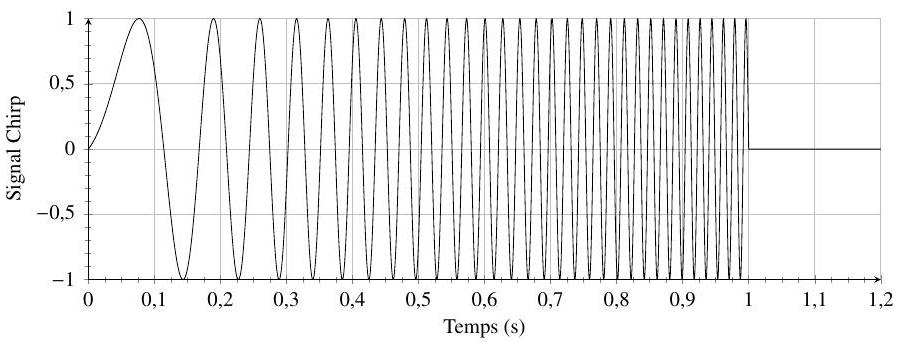
\includegraphics[max width=\textwidth]{2022_02_02_1af495ea60fb42b668bfg-03}

Figure 1 - Exemple de signal émis de type CHIRP

Q2. Écrire une fonction chirp(temps, fQ, Deltafe, T, EQ) qui renvoie un vecteur de taille $\mathrm{N}$ correspondant au signal émis défini sur $\left[0, T_{f}[\right.$ avec temps le vecteur défini précédemment et fQ , Deltafe, T, EO les paramètres intervenant dans le système d'équations définissant $e(t)$.

La réponse obtenue après réflexion sur un obstacle est de la forme donnée sur la figure $\mathbf{2}$.

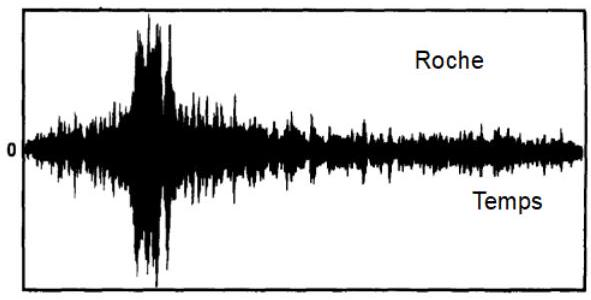
\includegraphics[max width=\textwidth]{2022_02_02_1af495ea60fb42b668bfg-03(1)}

Figure 2 - Exemple de signal de retour (extrait de travaux de recherche)

Pour analyser ce signal et notamment savoir sur quel type de support a eu lieu la réflexion, une transformation de Fourier (discrète) est pertinente car elle permet de connaître les composantes fréquentielles importantes dans le signal. Cependant, compte tenu des bruits et de la localisation du signal de retour, on préfère utiliser une transformation de Fourier dite locale qui consiste à appliquer la transformée de Fourier non pas sur tout l'intervalle de temps d'étude mais uniquement sur plusieurs courtes périodes temporelles qui se chevauchent.

\section{Description de l'algorithme de transformée de Fourier locale}
On note $s_{r}(t)$ le signal temporel de retour mesuré après réflexion sur l'obstacle. Le signal numérique correspondant est représenté par un vecteur de taille $N$ noté $\mathrm{s}$. La période d'échantillonnage de ce signal est $t_{e}=\frac{T_{f}}{N}$.

Pour obtenir les intervalles de temps utilisés dans la méthode, on sélectionne un instant particulier $(\tau)$ et $n<N$ instants. Ces instants seront répartis autour de la valeur $\tau$ ( $n / / 2$ avant et $n / / 2$ après). Pour extraire la portion de signal intéressante, on multiplie $s_{r}(t)$ par une fonction particulière qui peut être un simple créneau centré autour de $\tau$ ou des fonctions mathématiquement plus intéressantes comme celle de la figure 3 (fonction de Hamming).

En appliquant la transformée de Fourier (FFT) au signal obtenu, on extrait un vecteur de fréquences de taille $n_{f}=N / /(n / / 2)$ et un vecteur de nombres complexes (de taille $n_{f}$ ) dont le module correspond au spectre de Fourier. On répète le processus en décalant l'intervalle de temps sélectionné de $n / / 2$ valeurs (pour un chevauchement de $50 \%$ ).

Finalement, on obtient alors une fonction discrète de deux variables $S(f, t)$ où $f$ est un vecteur de fréquences de taille $n_{f}$ (le même pour toutes les fenêtres), $t$ est un vecteur contenant les valeurs de $\tau$ retenues de taille $n_{f}$ et $S$ l'ensemble des modules pour chaque fréquence et chaque instant $\tau$. Le tracé du module de $S$ en fonction des deux vecteurs $f$ et $t$ est appelé spectrogramme (figure 4).

Signal à analyser

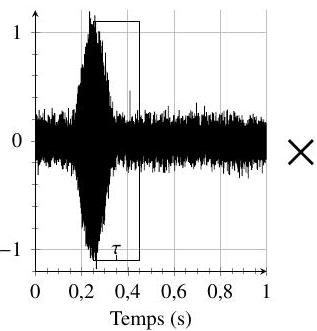
\includegraphics[max width=\textwidth]{2022_02_02_1af495ea60fb42b668bfg-04}

Fonction de Hamming

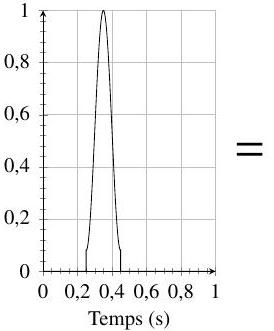
\includegraphics[max width=\textwidth]{2022_02_02_1af495ea60fb42b668bfg-04(1)}

Signal fenêtré

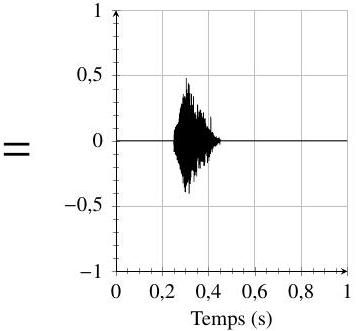
\includegraphics[max width=\textwidth]{2022_02_02_1af495ea60fb42b668bfg-04(2)}

Figure 3 - Principe de la transformée de Fourier locale d'un signal : sélection d'une partie du signal autour de $t=\tau$ en multipliant le signal à analyser par une fonction de Hamming

La fonction stft utilisée pour réaliser la transformée de Fourier locale est disponible dans le module scipy . signal. Un extrait de la documentation est proposé sur la page suivante.

Q3. À partir des indications précédentes et de la documentation, donner l'instruction permettant de stocker dans les variables notées $\mathrm{f}, \mathrm{t}, \mathrm{S}$ le résultat de la transformée de Fourier discrète du signal numérique s en précisant bien les arguments retenus, sachant que l'on souhaite un recouvrement de $50 \%$, que le nombre de valeurs retenues autour de chaque instant est $n$ et qu'on choisit une fenêtre de type Hamming. Donner également la taille des grandeurs $f, t$, $\mathrm{S}$ obtenues en retour en fonction de $n$ et $N$.

\section{Description de la fonction stft}
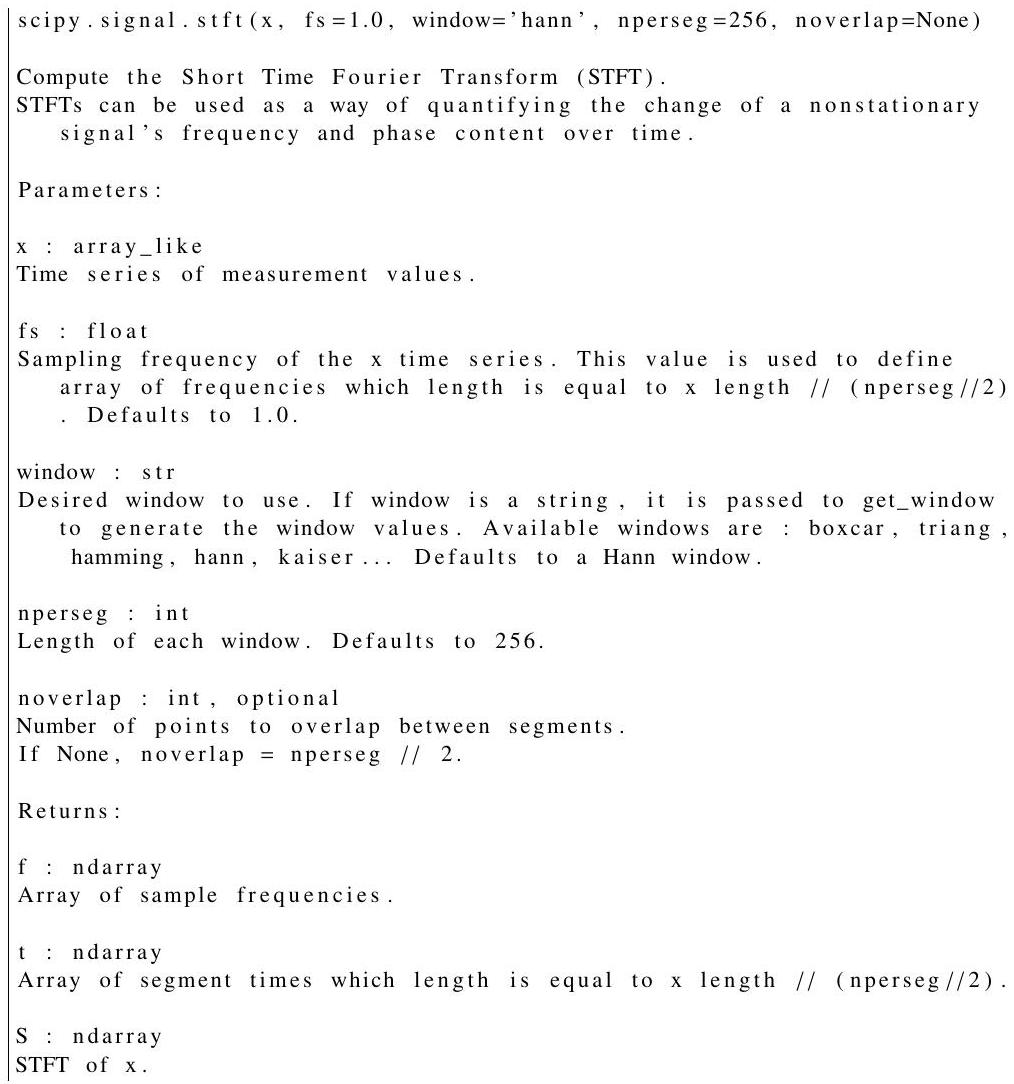
\includegraphics[max width=\textwidth]{2022_02_02_1af495ea60fb42b668bfg-05}

On teste la fonction sur le signal à analyser de la figure 3. Ce signal, qui a la même allure qu'une mesure expérimentale, a été construit à partir d'une fonction mathématique à laquelle un bruit a été rajouté.

Les spectrogrammes obtenus sont donnés sur la figure $4 .$ Q4. Commenter l'intérêt du spectrogramme pour analyser le contenu fréquentiel du signal d'origine et analyser succinctement la répartition obtenue entre $\mathrm{f}$ et $\mathrm{t}$.\\

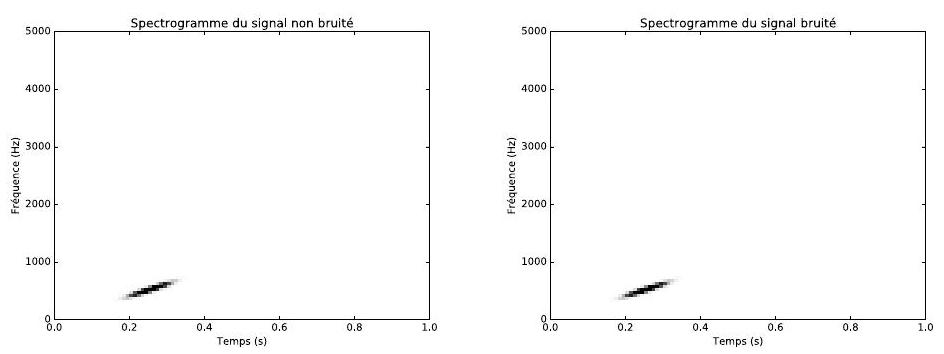
\includegraphics[max width=\textwidth]{2022_02_02_1af495ea60fb42b668bfg-06}

Figure 4 - Spectrogramme d'un signal bruité et d'un signal non bruité

Pour pouvoir comparer les résultats d'essais entre eux, il est préférable d'extraire l'enveloppe des spectrogrammes. Pour cela, on réalise une intégration numérique du signal tracé sur le spectrogramme : $P(\eta)=\int_{t} \int_{f} S(t, f) w(t, f, \eta) \mathrm{d} f \mathrm{~d} t$ avec $S(t, f)$ la fonction issue de l'analyse par transformée de Fourier locale et $w$ une fonction représentant un ensemble de fenêtres localisées autour de la zone d'intérêt dans le spectrogramme (de tailles $\Delta T$ et $\Delta f$ ). $\eta$ est un entier variant de 0 à $m-1$, permettant d'obtenir un ensemble fini de $m$ valeurs de l'enveloppe ( $m$ est un paramètre de l'analyse qui sera choisi par la suite).

On note $t_{\eta}=\frac{\Delta T}{2}+\eta T$ et $f_{\eta}=\frac{\Delta f}{2}+\eta \Delta f$.

La fonction $w(t, f, \eta)$ est définie par :
$$
\begin{cases}w(t, f, \eta)=1 & \text { si }-\Delta T / 2<t-t_{\eta}<\Delta T / 2 \text { et }-\Delta f / 2<f-f_{\eta}<\Delta f / 2 \\ w(t, f, \eta)=0 & \text { sinon }\end{cases}
$$
Q5. Écrire une fonction $w(t, f$, eta) qui renvoie 1 ou 0 en fonction des valeurs de $t, f$ et eta $=\eta$. On supposera que les paramètres $\Delta T, T$, et $\Delta f$ sont connus et utilisables directement dans la fonction (variables globales notées DT, T et Df).

On note $t_{i}$ les valeurs du temps, i variant de 0 à $n_{f}-1$ et $f_{j}$ les valeurs de fréquences, $\mathrm{j}$ variant de 0 à $n_{f}-1$ avec $t_{i}=i \mathrm{~d} t, f_{j}=j \mathrm{~d} f$ où $\mathrm{d} t \mathrm{et} \mathrm{d} f$ sont respectivement des pas de temps et de fréquence. La fonction à intégrer est notée $S_{i j}$ avec $i$ et $j$ variant respectivement de 0 à $n_{f}-1$ et 0 à $n_{f}-1$. Pour intégrer numériquement la fonction discrète $S_{i j}$, on utilise la formule : $P_{\eta}=\sum_{i} \sum_{j} p_{i j} S_{i j} w\left(t_{i}, f_{j}, \eta\right) \mathrm{d} f \mathrm{~d} t$ avec $p_{i j}$ poids (valeurs connues).

Q6. Écrire une fonction enveloppe (eta, $S, p, d t, d f$ ) qui renvoie la valeur de l'intégrale numérique en fonction de la valeur de eta $=\eta$. On supposera connus les pas $\mathrm{d} t$ et $\mathrm{d} f$. Le tableau numpy $S$ contient les valeurs de la fonction discrète $S_{i j}$ et le tableau numpy $\mathrm{p}$ contient les valeurs des poids $p_{i j}$. Pour chaque expérience (fonction de l'obstacle et de l'angle d'incidence de l'onde émise), on construit cette enveloppe. En prenant $m=60$, on obient 60 valeurs qui caractérisent une expérience. Ces valeurs seront utilisées dans les algorithmes de prédiction décrits dans la suite pour classer une nouvelle mesure.

De manière à pouvoir comparer les enveloppes, on normalise le vecteur $P_{\eta}$ en ramenant le maximum à 1 et le minimum à 0 par une fonction affine.

Q7. Proposer une fonction normalisation(P) qui renvoie un vecteur de $m$ valeurs comprises entre 0 et 1 . On pourra utiliser les fonctions $\min (\mathrm{x})$ et $\max (\mathrm{x})$ avec $\mathrm{x}$ un vecteur.

\section{II.2 - Lecture des données}
Les données à utiliser sont stockées dans un fichier texte où une ligne représente l'ensemble des valeurs associées à une expérience. Une expérience est caractérisée par 60 valeurs issues du traitement de la mesure (chaque valeur est un nombre réel entre 0 et 1) et un caractère donnant le groupe d'appartenance (un caractère $\mathrm{M}$ pour métal et $\mathrm{R}$ pour roche).

Premières lignes partielles du fichier, les points de suspension permettent de cacher les 56 données intermédiaires pour chaque ligne :

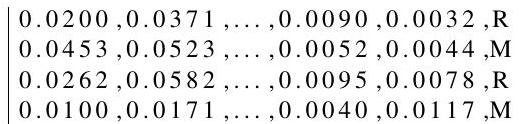
\includegraphics[max width=\textwidth]{2022_02_02_1af495ea60fb42b668bfg-07}

On souhaite lire ce fichier de données pour créer un tableau de type liste contenant des listes. Pour la dernière colonne, le caractère " $R$ ", respectivement " $M$ ", sera converti en la valeur $0.0$, respectivement 1.0. La fonction suivante permet de lire le fichier de données et renvoie les données au format souhaité.

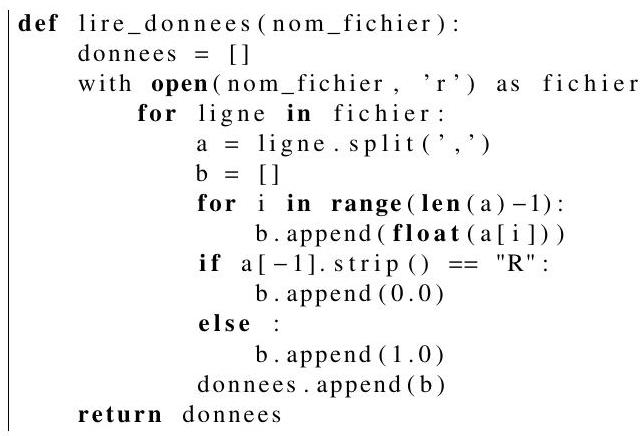
\includegraphics[max width=\textwidth]{2022_02_02_1af495ea60fb42b668bfg-07(1)}

Q8. À partir de la fonction lire\_donnees, préciser la valeur de la variable donnees en se limitant aux deux premières lignes lues. Les fonctions usuelles sur les fichiers et chaînes de caractères et leur documentation sont rappelées dans l'Annexe.

Le fichier de données comporte $n_{x}=208$ enregistrements.

Q9. Donner la taille mémoire minimale nécessaire en octets pour stocker les données. On rappelle que Python stocke les nombres réels en format double précision par défaut.

\section{Partie III - Méthode des forêts aléatoires}
La méthode des forêts aléatoires est une amélioration de la méthode des arbres de décision.

\section{III.1 - Arbre de décision}
Un arbre de décision est une représentation qui permet de séparer les données en deux groupes, appelés nœuds de l'arbre, selon un critère objectif. Les sous-groupes (ou nœuds) sont ensuite séparés en deux selon un autre critère, puis on sépare à nouveau jusqu'à obtenir un nœud terminal appelé feuille.

Pour classer une nouvelle donnée, il suffit ensuite de suivre les différentes règles issues de la construction de l'arbre pour savoir dans quelle catégorie la placer.

Le principal problème rencontré est qu'un arbre de décision peut vite conduire à du surapprentissage si l'on tente de décrire parfaitement le jeu de données initial avec une donnée unique par feuille. Dans ce cas, il ne sera pas forcément possible de classer une nouvelle donnée. Il est donc souvent nécessaire d'arrêter la construction à un nombre maximal de séparations, on parle d'élaguer l'arbre.

Illustrons ces notions sur le jeu de données aléatoires suivant, la dernière colonne représentant le groupe d'appartenance :

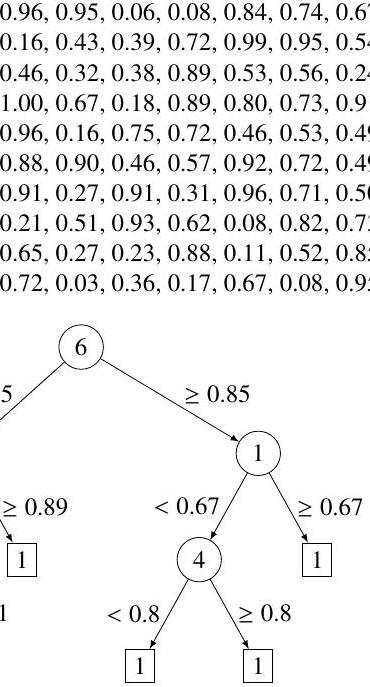
\includegraphics[max width=\textwidth]{2022_02_02_1af495ea60fb42b668bfg-08}

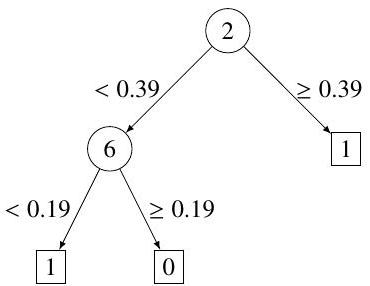
\includegraphics[max width=\textwidth]{2022_02_02_1af495ea60fb42b668bfg-08(1)}

(b) Exemple d'arbre de décision pour illustrer la représentation en Python

Figure 5 - Différents arbres de décision

Un arbre est représenté sur la figure 5(a). Cet arbre est composé de nœuds représentés par des cercles, des liens représentés par des flèches avec condition et des feuilles représentées par des rectangles composés de 1 ou de 0 . Un nœud contient l'indice d'une des colonnes du tableau de données (les colonnes sont numérotées à partir de 0). Les liens permettent de parcourir l'arbre de décision. Pour une ligne du tableau de données, on prend la valeur de la colonne d'indice indiqué par le nœud et on évalue la condition du lien. Si la valeur est strictement plus petite que la valeur indiquée sur le lien, on descend vers la gauche, sinon on va vers la droite. Lorsqu'on ne peut aller plus loin en descendant, on aboutit à une feuille représentant le type d'obstacle détecté ( 0 pour roche, 1 pour métal).

En Python, on choisit de représenter un nœud par une liste de 4 éléments [ind, val, gauche, droite]. Le premier élément est l'indice de la colonne du tableau de données, le deuxième élément est la valeur permettant de faire le test pour descendre à droite ou à gauche. Le troisième élément est :

\begin{itemize}
  \item soit le nœud de la branche de gauche (représentée elle-même par une structure de type nœud)

  \item soit la valeur terminale 0 ou 1 pour définir le groupe.

\end{itemize}
De même, le quatrième élément est soit le nœud de la branche de droite, soit la valeur terminale.

Par exemple, l'arbre de la figure $\mathbf{5}(\mathbf{b})$ sera représenté en Python par la liste suivante :

$[2, \theta .39,[6, \theta .19,1, \theta], 1] .$

Q10. Donner la représentation en Python de l'arbre défini sur la figure $\mathbf{5}(\mathbf{a})$.

Soit une donnée non classée $\mathrm{a}=[\theta .5, \theta .2, \theta .7, \theta .4, \theta .9, \theta .25, \theta .7, \theta .7, \theta .9, \theta .2]$.

Q11. Déterminer, en justifiant, dans quel groupe cette donnée sera classée en utilisant l'arbre de la figure 5(a). Expliquer le chemin parcouru dans l'arbre.

\section{III.2 - Construction d'un arbre}
Pour construire l'arbre, la principale question à laquelle il faut répondre est de savoir comment séparer les données à chaque itération. Il existe différentes méthodes, souvent statistiques, qui permettent de réaliser cette séparation. Nous allons ici étudier l'algorithme CART (« classification and regression trees »), qui se base sur une grandeur appelée indice de concentration de Gini qui sera définie par la suite. Cet indicateur permettra de choisir la colonne et la valeur pour faire la séparation.

La fonction suivante permet de séparer les données en deux groupes en utilisant l'indice de concentration de Gini. Nous allons détailler dans la suite les fonctions intervenant dans cette fonction. Pour rappel, la variable donnees est un tableau constitué de $n_{x}$ lignes et $m+1$ colonnes, la dernière colonne contient la classe à laquelle appartient la ligne (qui correspond à une expérience).

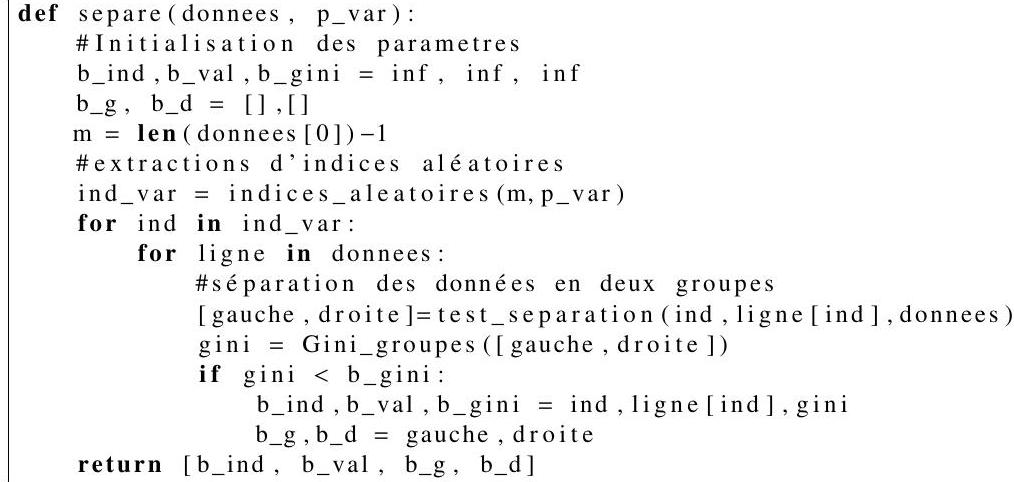
\includegraphics[max width=\textwidth]{2022_02_02_1af495ea60fb42b668bfg-09}

La fonction renvoie l'indice de la colonne et la valeur retenus pour faire le test de séparation ainsi que les deux groupes gauche et droite (la structure identique à la valeur renvoyée par la fonction lire\_donnees rappelée avant la question Q8).

Q12. Écrire une fonction indices\_aleatoires ( $m, p_{-} v a r$ ) qui prend en arguments le nombre $m$ correspondant au nombre de colonnes disponibles et p\_var un nombre permettant de tirer aléatoirement $p_{\text {var }}$ nombres parmi la liste des numéros de colonnes ( $\mathrm{p}_{-} \mathrm{var}<\mathrm{m}$ ) et qui renvoie une liste de taille $p_{\text {var }}$ contenant les numéros de colonnes tirés aléatoirement. Un numéro de colonne ne doit apparaître qu'une seule fois dans cette liste.

On utilisera la fonction randrange $(p)$ qui renvoie un entier aléatoirement entre 0 et $p-1$. Par exemple, si on choisit p\_var $=4$ avec $m=60$, on pourrait obtenir la liste d'indices aléatoires suivante $[10,50,3,24]$.

Q13. Écrire une fonction [gauche, droite]=test\_separation(ind, val, donnees) qui prend en argument ind un numéro de colonne, val une valeur permettant de séparer les données et donnees le tableau contenant les données. Cette fonction renvoie une liste de deux éléments du même type que donnees : les lignes, dont la valeur de la colonne ind est inférieure strictement à val, sont stockées dans le groupe gauche et les autres dans le groupe droite. Les groupes gauche ou droite peuvent être vides.

L'indice de concentration de Gini pour un jeu de données d'un groupe $g r$ (noté Gini $_{g r}$ ) est calculé à l'aide de la formule suivante : Gini $_{g r}=\sum_{i=0}^{k-1} 1-p_{i}^{2}$ où $k$ est le nombre de classes possibles, ici 2 (0 ou 1), $p_{i}$ est la proportion des éléments du jeu de données appartenant à la classe $i$. On rappelle que la valeur de la classe est contenue dans la dernière colonne du tableau de données.

Pour obtenir l'indice de concentration de Gini total pour les deux groupes (gauche et droite), on réalise une somme des deux indices de concentration Ginigr pondérée d'un coefficient de taille relative : taille du jeu de données du groupe divisé par le nombre de données des deux groupes (nombre de données totales).

Q14. Compléter les instructions notées 1 à 5 de la fonction Gini\_groupes donnée sur le document réponse qui prend en argument groupes la liste contenant les deux groupes à tester et qui renvoie l'indice de concentration de Gini.

Lors de la construction de l'arbre, on peut fixer plusieurs critères permettant d'arrêter la construction en calculant une feuille :

\begin{itemize}
  \item premier critère : quand le nombre de données à séparer est inférieur à une valeur que l'on notera taille\_min,

  \item deuxième critère : quand le nombre de séparations a atteint une valeur maximale notée sep\_max.

\end{itemize}
On donne à la feuille associée au jeu de données restant en fin de séparation la valeur du groupe majoritaire. Si la majorité des données est dans la classe 0 (roche) alors la feuille prendra la valeur 0 , sinon elle prendra la valeur 1 (métal).

Q15. Écrire une fonction feuille(data) qui prend en argument un jeu de données data et qui renvoie la valeur de la classe majoritaire. La variable data est du même format que la variable donnees.

La fonction permettant de lancer la construction de l'arbre est la suivante :

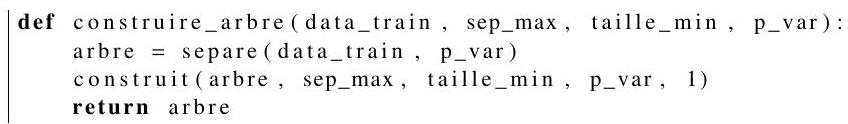
\includegraphics[max width=\textwidth]{2022_02_02_1af495ea60fb42b668bfg-10}

avec:

\begin{itemize}
  \item data\_train des données dont on connaît déjà la classe ;

  \item sep\_max : le nombre de séparations maximales pouvant être effectuées avant de placer une feuille ;

  \item taille\_min : le nombre de données minimales sous lequel on impose de mettre une feuille plutôt que de séparer les données en deux;

  \item p\_var : le nombre de valeurs à tirer aléatoirement pour le calcul de l'indice de concentration de Gini.

\end{itemize}
La construction de l'arbre est réalisée récursivement avec la fonction construit (arbre, sep\_max, taille\_min, p\_var, ind\_rec) après avoir créé un arbre initial à deux branches avec la fonction separe.

La fonction construit prend en argument entre autres :

\begin{itemize}
  \item arbre : structure de type noeud constituée de 4 éléments [ind, val, gauche, droite];

  \item sep\_max;

  \item taille\_min;

  \item p\_var;

  \item ind\_rec : l'indice de récursivité donnant le nombre de séparations déjà effectuées.

\end{itemize}
La fonction separe peut renvoyer un groupe gauche ou droite vide ([]), cela signifie qu'il n'y a pas eu de critères permettant de séparer les données en deux groupes. Dans ce cas, il faut calculer la feuille terminale associée au groupe non vide et imposer la valeur de cette feuille à droite et à gauche. Les variables gauche et droite peuvent être des nombres 0 ou 1 (feuilles) ou des structures de type nœud (cf. question Q10).

Dans la fonction récursive, la variable arbre de type nœud est modifiée au cours des appels successifs.

Q16. Compléter les conditions numérotées 1 à 4 de la fonction récursive construit donnée sur le document réponse.

\section{III.3 - Test d'une prédiction sur un arbre simple}
À partir des fonctions présentées précédemment, il est possible de construire un arbre de décision classique en prenant en compte toutes les colonnes disponibles pour faire les séparations. Pour le cas que l'on traite, on prendra ainsi p\_var $=60$.

Pour tester les performances de prédiction dans ce cas, on utilise un jeu de 100 données connues pour construire l'arbre. On réalise ensuite une prédiction sur un jeu de 50 données (non utilisées pour la construction mais dont on connait la classe) : pour chaque donnée, on parcourt l'arbre jusqu'à arriver sur une feuille qui donnera le groupe prédit. On compare cette prédiction à la classe connue. On compte le nombre de succès pour en déduire un taux de réussite. On recommence cette analyse en faisant une nouvelle construction d'arbre à partir des 100 données (ce qui correspond aux prédictions notées 1,2 et 3 ). On étudie également l'influence du nombre de données pour construire l'arbre en effectuant la même démarche pour des jeux de 125 et 150 données.

\begin{tabular}{|c|l|l|l|}
\hline
 & Arbre construit à partir de 100 données & Arbre construit à partir de 125 données & Arbre construit à partir de 150 données \\
\hline
Test de prédiction 1 & $79 \%$ & $74 \%$ & $88 \%$ \\
\hline
Test de prédiction 2 & $76 \%$ & $78 \%$ & $84 \%$ \\
\hline
Test de prédiction 3 & $74 \%$ & $78 \%$ & $77 \%$ \\
\hline
Temps moyen & $0,42 \mathrm{~s}$ & $0,64 \mathrm{~s}$ & $0,86 \mathrm{~s}$ \\
\hline
\end{tabular}

Tableau 1 - Pourcentages de réussite obtenus et temps de prédiction Le tableau 1 liste une synthèse des pourcentages de réussite obtenus ainsi que le temps pour réaliser une prédiction.

Q17. Au vu de ces quelques résultats d'analyse de la méthode des arbres de décision, indiquer de quels problèmes semblent souffrir cette méthode.

\section{III.4 - Algorithme des forêts aléatoires : « random forest »}
Pour palier les problèmes observés précédemment, on utilise un algorithme des forêts aléatoires. L'idée de l'algorithme des forêts aléatoires est de construire plusieurs arbres de décision (n\_arbres) basés sur une vision partielle du problème en se limitant à quelques variables (d'où l'introduction de la fonction indice\_aleatoire dans la partie précédente). En pratique, on utilise la racine carrée du nombre de variables, soit 7 au lieu de 60 dans notre exemple.

Ensuite, on réalise une prédiction sur les différents arbres construits et on associe à la donnée à classer la classe majoritaire issue des différentes prédictions élémentaires.

On suppose que l'on dispose des fonctions : construire\_foret qui renvoie une liste d'arbres (non détaillée ici) et prediction qui pour un arbre connu et une donnée renvoie la valeur de sa classe.

Q18. Compléter les 4 instructions manquantes de la fonction récursive prediction(arbre, donnee) donnée sur le document réponse qui prend en argument un arbre de décision noté arbre de type nœud et une donnée à classer donnee. La fonction isinstance(var, type) renvoie True si var est du type type.

On note :

\begin{itemize}
  \item data\_train, les données d'entraînement de l'algorithme qui vont servir à construire les arbres ;

  \item data\_test, les données permettant de tester l'efficacité de l'algorithme en comparant le classement proposé par rapport à la valeur connue.

\end{itemize}
Q19. Écrire une fonction random\_forest (data\_train, data\_test, sep\_max, taille\_min, n\_arbres, p\_var) qui renvoie une liste contenant la classe de chaque donnée contenue dans la variable data\_test.

\section{Conclusion}
On réalise des tests de prédiction comme cela a été présenté en sous-partie III.3.

Le tableau 2 liste une synthèse des pourcentages de réussite obtenus ainsi que le temps pour réaliser une prédiction avec une forêt de 20 arbres.

\begin{tabular}{|c|l|l|l|}
\hline
 & Arbre construit à partir de 100 données & Arbre construit à partir de 125 données & Arbre construit à partir de 150 données \\
\hline
Test de prédiction 1 & $88 \%$ & $84 \%$ & $91 \%$ \\
\hline
Test de prédiction 2 & $91 \%$ & $86 \%$ & $91 \%$ \\
\hline
Test de prédiction 3 & $86 \%$ & $83 \%$ & $88 \%$ \\
\hline
Temps moyen & $0,23 \mathrm{~s}$ & $0,35 \mathrm{~s}$ & $0,5 \mathrm{~s}$ \\
\hline
\end{tabular}

Tableau 2 - Pourcentages de réussite et temps de prédiction pour une forêt de 20 arbres

Q20. Conclure sur l'intérêt de cet algorithme des forêts aléatoires.

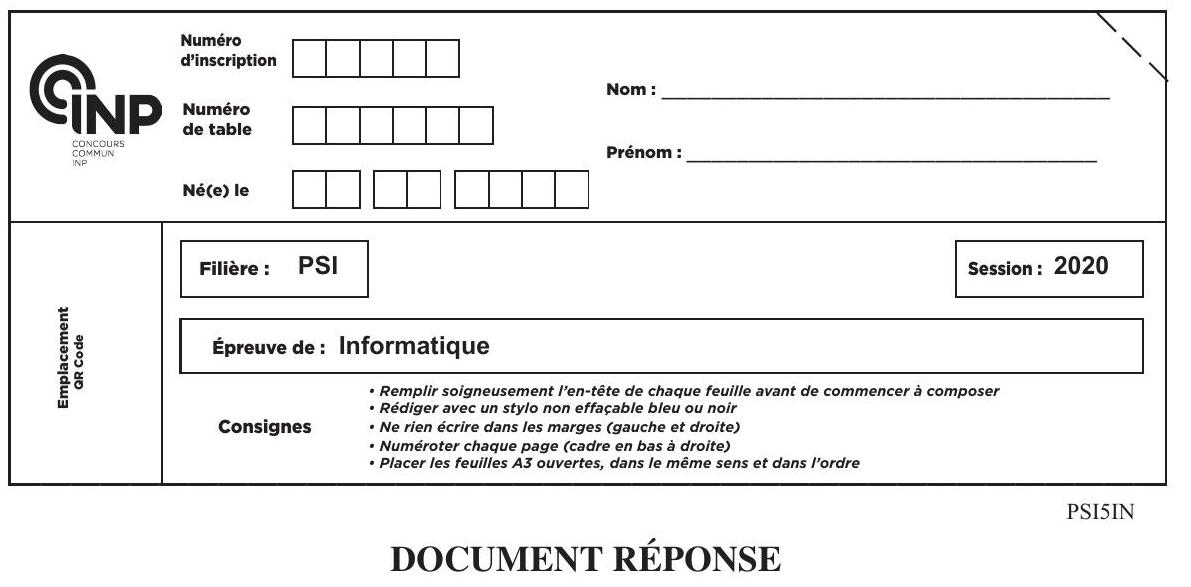
\includegraphics[max width=\textwidth]{2022_02_02_1af495ea60fb42b668bfg-13}

Q1 - Instruction pour la création de la variable temps

Q2 - Fonction chirp (temps, $f(\theta$, Deltafe, $\mathrm{T}$, $\mathrm{E} \theta$ )

Q3 - Instructions pour stocker $\mathrm{f}, \mathrm{t}$, S. Taille de $\mathrm{f}, \mathrm{t}, \mathrm{S}$ en fonction de $n$ et $N$

\section{NE RIEN ÉCRIRE DANS CE CADRE}
Q4 - Intérêt du spectrogramme

Q5 - Fonction w (t, f, eta)

Q6 - Fonction enveloppe (eta, $S, p, d t, d f$ ) Q7 - Fonction normalisation(P)

Q8 - Valeur de la variable donnees (deux premières lignes lues seulement)

Q9 - Taille mémoire minimale pour stocker les données

Q10 - Représention en Python de l'arbre de la figure $\mathbf{5}(\mathbf{a})$

Q11 - Classification de la donnée. Justification Q12 - Fonction indices\_aleatoires (m,p\_var)

Q13 - Fonction [gauche, droite] = test\_separation(ind, val, donnees)

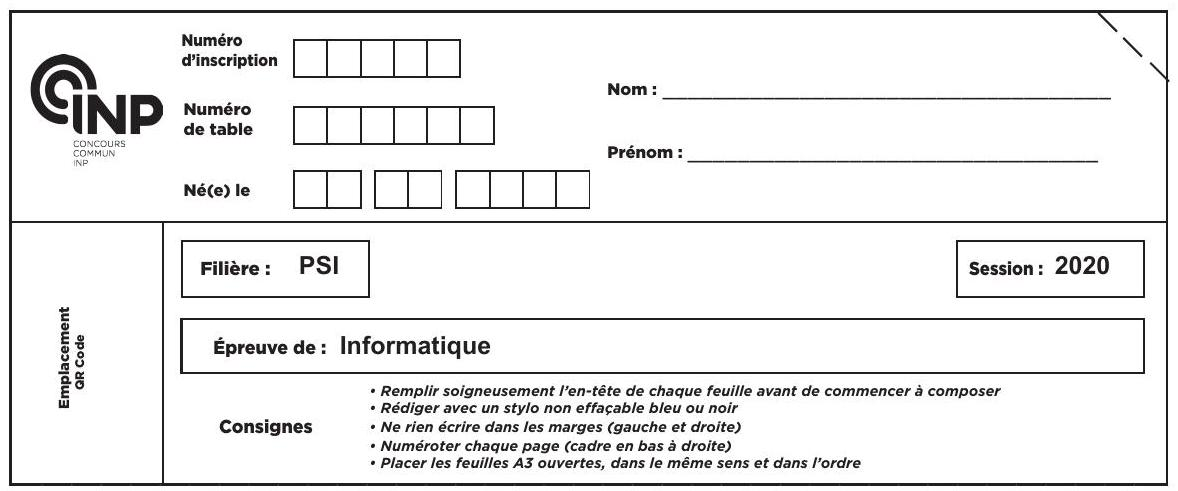
\includegraphics[max width=\textwidth]{2022_02_02_1af495ea60fb42b668bfg-17}

PSI5IN

Q14 - Compléter les instructions notées 1 à 5

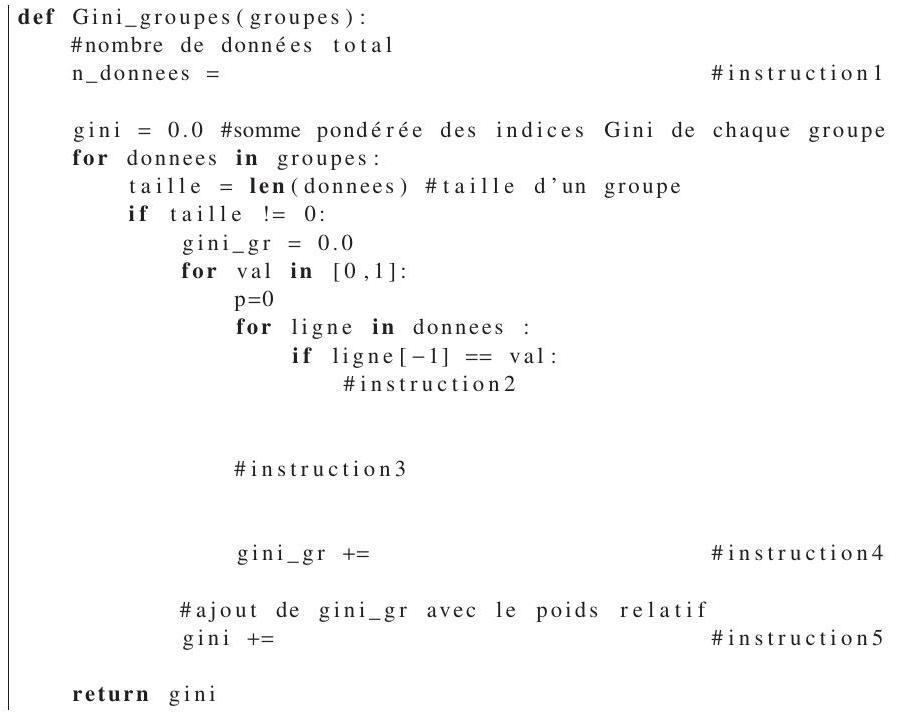
\includegraphics[max width=\textwidth]{2022_02_02_1af495ea60fb42b668bfg-17(1)}

\section{NE RIEN ÉCRIRE DANS CE CADRE}
\section{Q15 - Fonction feuille (data)}
Q16 - Compléter les conditions numérotées 1 à 4 de la fonction récursive construit

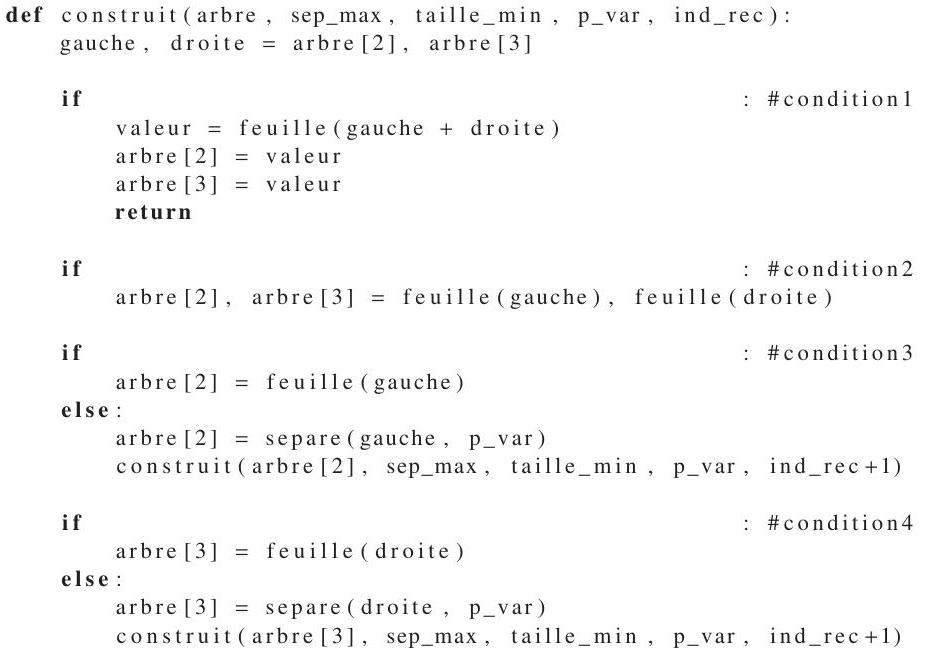
\includegraphics[max width=\textwidth]{2022_02_02_1af495ea60fb42b668bfg-18}

Q18 - Compléter les 4 instructions manquantes

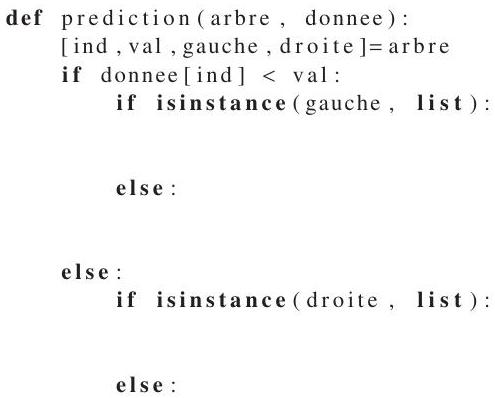
\includegraphics[max width=\textwidth]{2022_02_02_1af495ea60fb42b668bfg-19}

\#instruction 1

\#instruction 2

\#instruction 3

\#instruction 4

Q19- Fonction random\_forest (data\_train, data\_test, sep\_max, taille\_min, n\_arbres, p\_var) Q20 - Conclusion sur l'intérêt de l'algorithme des forêts aléatoires

\section{ANNEXE}
\section{Rappels des syntaxes en Python}
Remarque : sous Python, l'import du module numpy permet de réaliser des opérations pratiques sur les tableaux : from numpy import *. Les indices de ces tableaux commencent à $0 .$

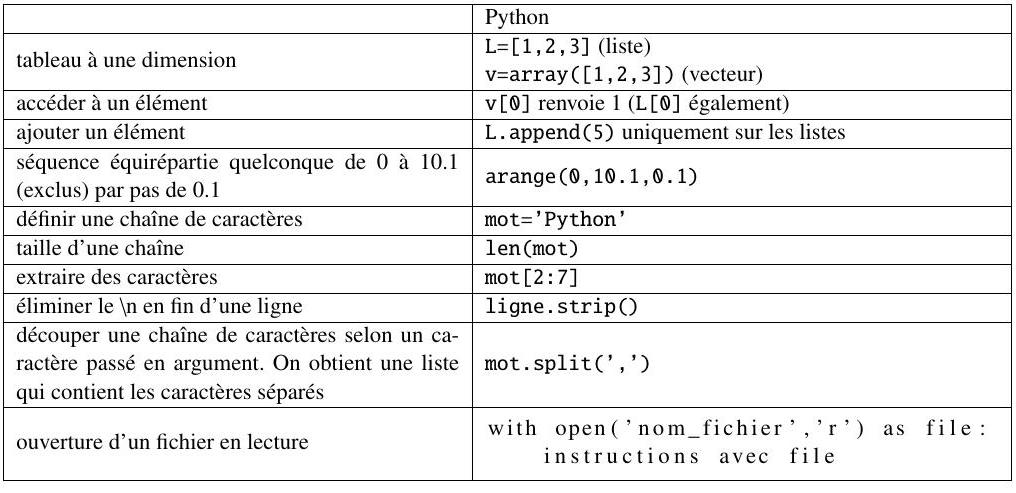
\includegraphics[max width=\textwidth]{2022_02_02_1af495ea60fb42b668bfg-20}


\end{document}